\cotefile{83}
\scanpage{194}
% archive sheet number: 193

(fonctions \deleted{symétriques} \inserted{\unsure{déterminantes|déterminants|déterminées}} pour l'action du groupe $\unsure{\mathfrak S|\mathscr S}_{\{i,j,k\}}\subset\mathfrak S_4$). \unsure{Ça|Si} fait qu'en fait, il suffit comme générateurs les quatre quantités (en plus du quatuor $b_{,,},c_{,,},t_{..}$ du début)

\[
 t_{2,3,4},\,t_{1,3,4},\,t_{1,2,4},\,t_{1,2,3}
\]

Si $A$ est l'anneau engendré par les $b_{..},c_{..},t_{..}$, je présume que $B$ est fini libre de rang $2^4$ sur $A$, avec $8$ \unsure{génér.} \inserted{distincts $t_{ijk}$} sur $A$ soumis aux seules relations $(\ast)$ ci-dessus.

Mais il faudrait trouver la relation entre les $b_{\unsure{j|i}},c_j,t_{k,\ell}$ -- peut-être via les $t_{ijk}$. La clef pour la trouver \deleted{\unsure{est}} \inserted{sera} le calcul de l'expression

\[
 \operatorname{Tr} x_1x_2x_3x_4
\]

\deleted{\unsure{,}}
\scanpage{195}
% archive sheet number: 194

% Reverse-side typescript shows through in mirror image.
\[
 \deleted{\beta'=-\beta}
\]

\[
 \begin{aligned}
 &\deleted{\unsure{,}\,bc'+b'c''+b''c}\\
 &\deleted{-(bc''+b'c+b''c')}
 \end{aligned}
\]

\[
 \deleted{\alpha'=}
\]

\[
 \deleted{\overline{\alpha^{\unsure{\prime|1}}}'=\bar\alpha+\beta\sigma}
\]

\[
 \mathbb Z \qquad \tau\tau'= \qquad \deleted{(\alpha-\bar\alpha)'=\alpha-\bar\alpha}
\]

\[
 \begin{aligned}
 &\deleted{b\,;c,t}\\
 &\deleted{b',c',t'}\\
 &\deleted{b'',c'',t''}
 \end{aligned}
\]

\[
 \alpha'-\alpha=\beta\sigma
\]

\figure{\begin{tikzpicture}[overlay,remember picture]
\draw[thin] (-3.6,-3.1) .. controls (-3.5,-0.4) and (-2.8,0.4) .. (-0.7,0.45) .. controls (0.6,0.44) and (2.8,0.50) .. (3.25,-0.6) .. controls (4.1,-2.0) and (4.05,-3.4) .. (3.5,-5.5);
\end{tikzpicture}}

$A$\qquad $\unsure{\mathfrak S|\mathscr S}_3$ y opère, \unsure{fidèlt|fidlt}

\[
 b\unsure{-|\to|\mapsto}b'-b''\qquad c-c'-c''\qquad t-t'-t''
\]

\[
 \deleted{\unsure{\mathbb Z}}\quad
 \underline{\unsure{\mathbb O|\mathbb D|O|\mathbb A}^{3}}\times\underline{\mathbb O^{3\unsure{\prime}}}\times\underline{\mathbb O^{3}}\qquad\ldots
\]

\margin{Fonctions $G$-invariantes en $3$ variables $x,y,z$}

\diagram{\begin{tikzcd}[ampersand replacement=\&,column sep=large,row sep=small]
 \& B \& \\
 \& A\arrow[u]\arrow[r,dash,"\mathfrak S_2"] \& B\\
 \unsure{a|\leftarrow|-}\& A^{\mathfrak S_3}\arrow[u,dash,"\mathfrak S_3"']\arrow[r,dash,"\mathfrak S_2"'] \& B_0\arrow[u,dash,"\mathfrak S_3"']\\
 \& \deleted{\unsure{B|k}}\mathbb Z[\Sigma,\Pi]\arrow[u,dash]\arrow[r,dash] \& B_{00}\arrow[u,dash]
\end{tikzcd}}

$\mathfrak S_3\times\mathfrak S_2$ opère sur $B$ \quad inv. \quad $A^{\mathfrak S_3}$

\[
 \unsure{\tfrac26}\qquad \mathfrak S_3\underset{(\mathrm{id},\mathrm{sg})}{\unsure{-|\longrightarrow}}\mathfrak S_3\times\mathfrak S_2
\]
\scanpage{196}
\mspage{L 19}
% archive sheet number: 195

que en l'occurence) ne s'apparente pas au pur travail du marteau sur l'enclume ou sur le burin\deleted{\unsure{er|e}} - le mépris des processus créateurs \inserted{\handwritten{les}} plus délicats (et \inserted{\handwritten{parfois}} de moindre apparence) , \deleted{et à la limite} de tout ce qui est \deleted{idée, vision,} inspiration, rêve , vision \deleted{ou \deleted{même} simplement idée, même si clairement conçue et formulée soit-elle} \inserted{\handwritten{si puissants et fertiles soient-ils}} \inserted{\handwritten{et même}} (à la limite) de toute \mbox{i\,d\,é\,e} , si clairement conçue et formulée soit-elle; de tout ce qui n'est écrit et \mbox{p\deleted{\unsure{u}}u\,b\,l\,i\,é} \unsure{noir|noit} sur blanc, sous forme d'énoncés purs et durs, \deleted{et avec démontrés,} \unsure{répertoriables|répertorizables|répertoriéables} et répertoriés, mûrs pour les ``banques de \uline{données''} s'engouffrant dans \deleted{\unsure{d'}}\inserted{les} inépuisables mémoires de nos mégaordinateurs.

Il y a eu \deleted{\illegible{1}} (pour reprendre \deleted{les} une expression de C.L. Siegel ($^{\ast}$)) un extraordinaire ``\uline{aplatissement}'' ou ``\uline{rétrécissement}'' dans la pensée mathématique($^{\ast}$), dépouillée d'une dimension essentielle, \deleted{d'un ``versant''} \inserted{\handwritten{de \deleted{tout} son}} \deleted{de son} ``versant\deleted{\unsure{''}} \inserted{\handwritten{d'ombre''}}, \deleted{\illegible{1}} \inserted{\handwritten{du versant}} \deleted{\illegible{1}} ``féminin''. \deleted{Traditionnellement,} \inserted{\handwritten{Il est vrai que de tradition ancestrale,}} ce versant-là \deleted{restait} \inserted{du travail de découverte} \deleted{scientifique} \inserted{restait} dans une large mesure occulté, \deleted{\unsure{dans la on n'en|dans les on n'en}} personne (autant dire) n'en \uline{parlait} jamais - mais le contact avec les sources profondes du rêve, qui alimentent \deleted{les grands desseins et} les grandes visions et les grands desseins, \deleted{\unsure{n'a jamais nté|n'a jamais été}} \inserted{n'avait} jamais \inserted{\handwritten{encore}} (à ma connaissance) était perdu. Il semblerait \deleted{que} \inserted{qu'à présent} nous sommes déjà entrés dans une époque \deleted{où ce contact est sur le point d'être} \inserted{de \mbox{d\,e\,s\,s\,é\,c\,h\,e\,m\,e\,n\,t},} \inserted{où} cette source est, non point tarie certes, mais où l'accès à elle est condamné\deleted{\unsure{e}}, par le verdict sans appel \deleted{de la dérision ed} du mépris \deleted{généraux} \inserted{général} et par les représailles de la dérision. Nous approchons du moment, \unsure{semble-tèil|semble-t-il}, où \inserted{\unsure{sera éradiqué|sesa éradiqué}} non seulement le \uline{souvenir} \inserted{\handwritten{en chacun}} \deleted{des stades et étapes} \inserted{de \deleted{ces} tout travail} \deleted{\unsure{à notre|d'une}} proche de la source, du travail \handwritten{à} \deleted{\unsure{lien à|lien a}} dominante ``féminine'', \deleted{dans le travail mathématique (stades} (ridiculisés par des épithètes comme ``vaseux'', ``mou\deleted{\unsure{s}}'', ``inconsistant\deleted{\unsure{s}}'' - \deleted{ou} au bout opposé, \deleted{``trivial'', ``évident'',} \inserted{``trivialités'', ``évidences'',} ``bombinage'' \deleted{de} ...), mais \inserted{\handwritten{où sera extirpé}} \deleted{des stades} \inserted{ce travail} \deleted{étapes elles-mêmes, celles qui où naissent les} \inserted{de gestation même: celui} où sont conçues, s'élaborent et naissent les notions et les visions nouvelles. \deleted{\unsure{Le} \handwritten{\unsure{que}}} \inserted{Ce sera} \inserted{aussi} où l'exercice de notre art sera réduit à \deleted{\unsure{un|de}}\handwritten{\unsure{de|un}} \inserted{\unsure{aride|ar}\handwritten{\unsure{de|le}}} exercice de ``poids et haltères''\inserted{cérébral} - ce\handwritten{lle} d'une hypertrophie \inserted{fiévreuse et} stérile, prenant la suite de plus de trois siècles \deleted{\unsure{de|ce}}\inserted{\handwritten{\unsure{d'i|dit|d'}}} renouvellement créateur...

Mais à nouveau je \deleted{anticipe ou} digresse, \deleted{\unsure{ou}} j'anticipe sur ce que la réflexion m'a enseigné, \deleted{dans la en continu} \inserted{\handwritten{en partant}} \deleted{dans la direction} d'un double propos clairement présent en moi \deleted{en commençant mon ``introduction'', en juin 1983 d'abord et en la reprenant en février l'année dernier (l'année d'après):} \inserted{\handwritten{dès avant même les débuts de \deleted{\illegible{1}} celui-ci:}} le propos d'une ``déclaration d'intentions'', et (intimement lié à celui-ci) celui de m'exprimer au sujet de \deleted{\unsure{b}}\unsure{la} nature du travail créateur. Il y avait pourtant un troisième propos encore, moins clairement présent sûrement au niveau conscient, mais correspondant à un besoin plus profond
\scanpage{197}
% archive sheet number: 196

\[
 \operatorname{Tr}u^n=P_n(\operatorname{Tr}u,\deleted{\unsure{\}}}\det u)
\]

\[
 \operatorname{Tr}u^{n_1}v^{m_1}u^{n_2}v^{m_2}\mathord{\text{---}}u^{n_r}v^{m_r}
 =P_{(n_1,m_1,n_2m_2,\mathord{-}\,\mathord{-}\,n_r,m_r)}(
\]

\[
 \lambda^n+\mu^n=P_n(\lambda+\mu,\lambda\mu)
\]

\[
 \operatorname{Tr}x_1x_2x_3x_4=\operatorname{Tr}x_1x_2(x_3x_4)
\]

\[
 \deleted{\unsure{t_{12}}-t_{1234}^{2}-\Sigma_{1,2,(3,4)}t_{1234}-}
\]

\[
 \tau^2-\Sigma_{1,2,(3,4)}\tau+\Pi_{1,2,(3,4)}=0
\]

$\Sigma_{1,2,(3,4)},\Pi_{1,2,(3,4)}\in\deleted{\mathbb Z[b_1,c_1,b_2,c_2,}$ expression pol. à coeff. entiers en

\[
 \begin{aligned}
 &\underbrace{\operatorname{Tr}x_1}_{\substack{\unsure{\text{''}|\mathrm{II}}\\ b_1}},\ \underbrace{\det x_1}_{c_1},\
 \underbrace{\deleted{\unsure{\mathrm d}}\operatorname{Tr}x_2}_{b_2},\
 \underbrace{\det x_2}_{c_2},\quad\underbrace{\operatorname{Tr}x_3x_4}_{t_{3,4}},\
 \underbrace{\det(x_3x_4)}_{c_3c_4}\\
 &\underbrace{\operatorname{Tr}x_1x_2}_{t_{12}},\
 \underbrace{\operatorname{Tr}x_2(x_3x_4)}_{t_{2,3,4}},\
 \underbrace{\operatorname{Tr}(x_3x_4)x_1}_{t_{134}}
 \end{aligned}
\]

donc dans

\[
 \mathbb Z[b_1,c_1,b_2,c_2,c_3,c_4,t_{1,2},
 \underset{\unsure{9|q}}{\underline{t_{2,3,4}}},t_{1,3,4}]
\]

entier sur

\[
 \begin{aligned}
 \mathbb Z[&b_1,c_1,b_2,c_2,b_3,c_3,b_4,c_4,t_{1,2},t_{1,3},t_{1,4},\\
 &t_{23},t_{24},t_{24}]
 \end{aligned}
\]

$\tau$ de degré au plus huit sur $A$ ('' divisant '')
\scanpage{198}
\mspage{L 17}
% archive sheet number: 197

entrevu seulement et encore moins vu et touché, pour peu à peu se \deleted{dégager de son manteau de brumes, et se} \deleted{\inserted{d'ombre et}} décanter de l'impondérable, se dégager de son manteau d'ombre et de brumes et prendre forme et chair. \deleted{Ce sont} \inserted{C'est} \deleted{ces stades} \inserted{cette partie}-là du travail, de piètre apparence pour ne pas dire foireux, qui \deleted{\unsure{en représentent aussi les plu|en représentent aussi les plus|à y regarder de plus près}} \inserted{en \deleted{sont} est aussi la plus} névralgique - celle où, véritablement quelque chose de \mbox{n\,o\,u\,v\,e\,a\,u} fait son apparition, par l'effet d'une attention intense, d'une sollicitude, d'un respect pour cette chose fragile, infiniment délicate, sur le point de naître. C'est la partie créatrice entre toutes - celle\deleted{\unsure{s}} de la conception et de la gestation d'un \unsure{fragile|gragile} embryon dans \unsure{hes|les} chaudes ténèbres de la matrice nourricière, \deleted{élaborant en silence} depuis l'invisible double gamète \deleted{initiale} originelle devenant embryon et se transformant au fil des jours et des mois, par un travail obscur et intense, \unsure{irvisible|invisible} et sans apparence, en un nouvel être en chair et en os.

\unsure{C'est|Cest} là aussi la partie \inserted{éminemment} ``yin'', ``féminine\deleted{\unsure{,}}'' du travail de découverte - alors que \deleted{la partie} l'aspect complémentaire ``yang'', ou masculin, s'apparenterait plutôt \deleted{\unsure{aux|auxx}} au travail à coups de marteaux ou de masse, sur un burin bien affûté ou sur un coin de bon acier trempé. L'un et l'autre aspect a sa raison d'être et sa fonction, en symbiose inséparable \inserted{l'un} avec l'autre - ou pour mieux dire, ce sont là \uline{l'épouse} et \uline{l'époux} du couple des deux forces cosmiques originelles, dont l'étreinte \deleted{\inserted{sans cesse} renouvelée fait} sans cesse renouvelée fait resurgir sans cesse les obscurs labeurs créateurs de la conception, de la gestation et de la naissance - de la naissance de \mbox{l'\,e\,n\,f\,a\,n\,t} , de la chose nouvelle.

La deuxième chose sur laquelle je sentais le besoin de m'exprimer, dans ma fameuse ``introduction'' \deleted{philosophique et} personelle et ``philosophique'' à un texte mathématique, c'était au sujet de la nature du travail créateur justement. Je me rendais compte, depuis des années, que cette nature était généralement \unsure{ignorée|ngnorée}, occultée par des clichés à tout venant et par des peurs ancestrales. A quel point il en est bien ainsi, je l'ai découvert \unsure{progressivement|progressigement}, \unsure{au|an} fil des jours et des mois, tout au cours de la réflexion et de ``l'enquêté'' poursuivie dans Récoltes et Semailles. C'est dès les tout débuts de cette réflexion, au mois de juin 1983, que je suis saisi pour la \unsure{première|premmère} fois (pour l'oublier \inserted{un peu} par la suite ...) par la portée de ce fait d'anodine apparence, et pourtant asses stupéfiant, pour peu seulement qu'on s'y arrête tant soit peu: que cette partie ``créatrice entre toutes'' dont je viens de parler dans le travail de découverte, \uline{ne transparaît pratiquement nulle part} dans les textes qui sont censés
\scanpage{199}
% archive sheet number: 198

\[
 \tau=\operatorname{Tr}(x_1x_2)x_3x_4\qquad x_2x_1
\]

\figure{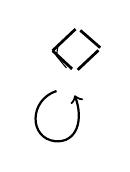
\begin{tikzpicture}[scale=.55]
\draw[line width=1pt] (0,1.4)--(.53,1.9) (.64,1.87)--(1.1,1.47) (1.06,1.41)--(.58,.96) (.45,.98)--(0,1.4);
\draw (.12,1.5)--(.09,1.28)--(.32,1);
\draw[->,line width=.8pt] (.09,.47) .. controls (-.55,.26) and (-.55,-.62) .. (.06,-.69) .. controls (.56,-.73) and (.72,-.2) .. (.51,.37);
\end{tikzpicture}}

\figure{
\begin{tikzpicture}\draw[line width=1.8pt] (0,0)--(.45,.02);\fill (.65,.08) circle (.012) (.9,.10) circle (.012);\end{tikzpicture}}

\[
 \tau^2-\Sigma_{(1,2),3,4}\tau+\Pi
\]

\[
 \operatorname{Tr}x_1x_2x_3\deleted{\unsure{x}}x_4+\operatorname{Tr}x_2x_1x_3x_4
\]

\[
 \begin{aligned}
 &x_1x_2x_3x_4 &x_2x_3x_4x_1&&x_3x_4x_1x_2 &x_4x_1x_2x_3\\
 &x_4x_3x_2x_1 &x_3x_2x_{\unsure{1|.}}\\
 &&&&\tau
 \end{aligned}
\]

\figure{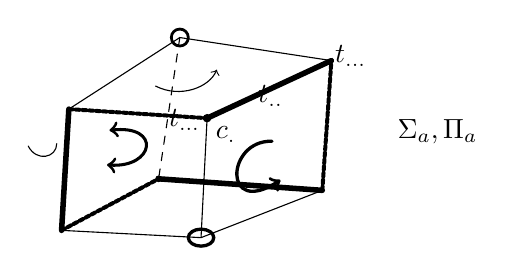
\begin{tikzpicture}[scale=.77,line cap=round]
\coordinate (a) at (0,0); \coordinate (b) at (2.3,-.12); \coordinate (c) at (4.3,.66); \coordinate (d) at (1.6,.85);
\coordinate (e) at (.12,2); \coordinate (f) at (2.4,1.85); \coordinate (g) at (4.45,2.8); \coordinate (h) at (1.95,3.18);
\draw (a)--(b)--(c)--(g)--(h)--(e)--(f)--(b);
\draw[line width=2pt] (a)--(e) (f)--(g) (d)--(c);
\draw[dashed] (h)--(d); \draw[densely dotted,line width=1.45pt] (a)--(d) (e)--(f) (c)--(g);
\draw[line width=1pt] (h) circle (.14); \draw[line width=1.2pt] (b) ellipse (.21 and .14);
\fill (f) circle (.07) (d) circle (.055);
\draw[->] (1.55,2.38) .. controls (1.96,2.17) and (2.44,2.36) .. (2.56,2.65);
\draw[<->,line width=1.1pt] (.75,1.08) .. controls (1.53,1.02) and (1.66,1.75) .. (.79,1.65);
\draw[->,line width=1.2pt] (3.47,1.47) .. controls (2.71,1.49) and (2.65,.20) .. (3.61,.83);
\draw (-.55,1.39) .. controls (-.41,1.12) and (-.08,1.2) .. (-.08,1.43);
\node at (2.03,1.82) {$t_{\ldots}$}; \node at (2.71,1.58) {$c_{.}$}; \node at (3.45,2.21) {$t_{..}$}; \node at (4.77,2.87) {$t_{\ldots}$};
\node at (6.2,1.63) {$\Sigma_a,\Pi_a$};
\end{tikzpicture}}

\[
 \deleted{\unsure{\tau^2-}}\qquad \tau^2
\]

\[
 \underline{b_s,c_s},t_s\ \big|\ \underline{t_a}\ \big|\ t_f
\]

\[
 \tau^{\unsure{\infty|8}}+\alpha_1\tau^7\mathord{\text{---}}+\alpha_8=0
\]

\uline{Nb} $\left\{\begin{aligned} b_s&=b_{s'}\\c_s&=c_{s'}\\t_a&=t_{a'}\end{aligned}\right.$

\[
 \alpha_i\in\mathbb Z[b_{..},\unsure{c_{.}},t_{..}]
\]

mais $\left\{\begin{aligned}t_s&\ne t_{s'}\\t_f&\ne t_{\unsure{f\,f'|f'}}\end{aligned}\right.$ \quad de degré $2$ sur $A^{\unsure{\mathfrak S|\mathscr S}_4}$\\ de degré $8$ sur $A^{\mathfrak S_4}$\\ \uline{de degré $6$ sur $B^{\mathfrak S_4}$}\\ de degré $8$ (?) \deleted{\unsure{?}} sur $A$

\[
 \begin{aligned}
 &g\unsure{\tau_+|x_+|\tau},\ g'\tau\quad g''\tau\\[-1pt]
 &\Sigma g\tau\\[-1pt]
 &\Sigma g
 \end{aligned}
\]

\[
 \begin{aligned}
 &\tau^\infty+\beta_1\tau^7\mathord{\text{---}}+\beta_8=0\\
 &\underbrace{(\alpha_1-\beta_1)}_{\gamma_1}\tau^7\mathord{\text{---}}+\underline{\alpha_8-\beta_8}=0
 \end{aligned}
\]

\figure{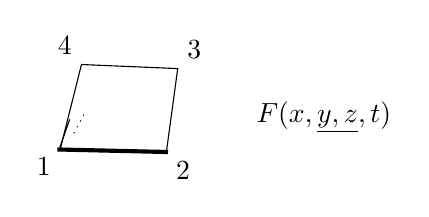
\begin{tikzpicture}[scale=.65]
\draw (.06,.12)--(.47,1.75)--(2.35,1.67)--(2.13,.05);
\draw[line width=1.5pt] (0,.09)--(2.16,.04); \draw (.05,.14)--(.24,.68); \draw[dotted] (.32,.41)--(.56,.85);
\node[above left] at (.47,1.75) {$4$};\node[above right] at (2.35,1.67) {$3$};\node[below left] at (.06,.12) {$1$};\node[below right] at (2.13,.05) {$2$};
\node[right] at (3.7,.71) {$F(x,\underline{y,z},t)$};
\end{tikzpicture}}

\[
 H\subset\mathfrak S_4
\]

\diagram{\begin{tikzcd}[ampersand replacement=\&,row sep=small]
 B^H\arrow[d,dash,"\text{degré }6"]\\ B^{\mathfrak S_4}=B^G
\end{tikzcd}}

$\alpha+\beta\tau\qquad a\quad b$ stables par $\unsure{+\mathfrak S_3^+|\mathfrak S_3^+}$

\[
 \begin{aligned}
 &\text{''}\quad\alpha'+\beta'\tau'=\alpha'+\beta'(\sigma-\tau)=(\alpha'+\beta'\sigma)-\beta'\tau\\
 &\beta'=-\beta\ /\ \alpha'\unsure{+|-}\beta\sigma=\alpha\qquad
 \alpha'=\alpha+\beta\sigma\ /\ (\alpha')'=\alpha=\alpha'+
 \end{aligned}
\]
\scanpage{200}
% archive sheet number: 199

\handwritten{\diagram{\begin{tikzcd}[ampersand replacement=\&,row sep=small,column sep=small]
 A\arrow[rr,Rightarrow] \& \& B\\
 A^{\unsure{\mathfrak S|\mathscr S}_3^+}\arrow[u,"3"]\arrow[rr,dash,"2"] \& \& B_1=B^{\mathfrak S_3^+}\arrow[u,dash,"3"']\\
 \& B^{\mathfrak S_3}\arrow[ur,dash] \& \\
 A^{\mathfrak S_3}\arrow[uu,"2"]\arrow[ur,dash]\arrow[rr,dash,"2"] \& \& B_{\unsure{0|\circ}}\arrow[uu,dash,"2"']
\end{tikzcd}}}

\handwritten{\[
 \begin{aligned}
 &\alpha+\beta\tau+\alpha'+\beta'\tau'\\
 &=(\alpha+\alpha')+\bigl(\beta\tau+\beta'(\sigma-\tau)\bigr)\\
 &=\underline{\alpha+\alpha'}+\underline{\beta'\sigma}+(\beta-\beta')\tau
 \end{aligned}
\]}

\handwritten{\[
 \alpha+\alpha'+\beta\sigma-(\alpha+\alpha'+\beta'\sigma)=(\beta-\beta')\sigma\qquad\mathrm{OK}
\]}

% Typed passage runs sideways relative to the handwritten calculations.
\mspage{L 22}

% Black shape touching the j; shown in the reading direction of the type.
\figure{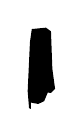
\begin{tikzpicture}[x=.58cm,y=.58cm]
\fill (0,0)--(-.03,.37)--(.02,1.45)--(.06,1.73)--(.37,1.76)--(.48,1.68)--(.51,.86)--(.57,.42)--(.48,.33)--(.41,.34)--(.33,.15)--(.20,.09)--(.04,.12)--(.04,-.02)--cycle;
\end{tikzpicture}}

Tout ce que \unsure{je} croyais avoir à dire, à un moment ou à un autre\deleted{\unsure{s|d}} de la réflexion, \handwritten{(}que ce soit sur moi, ou sur tel autre, ou sur un milieu, ou sur une époque, je l'ai dit, sans \inserted{jamais} avoir à bousculer mes réticences. Il a suffi à chaque fois que je les examine avec attention, pour qu'elles s'évanouissent\deleted{\unsure{,|.}} sans plus laisser de traces.
\scanpage{201}
% archive sheet number: 200

\[
 \begin{aligned}
 \tau_f+\tau_{f'}&=\Sigma_a\\
 \tau_{f'}+\tau_{f''}&=\Sigma_{a'}
 \end{aligned}
\]

\[
 \begin{aligned}
 \longrightarrow\quad \tau_f-\tau_{f''}&=\Sigma_a-\Sigma_{a'}=\Sigma_{\bar a}-\Sigma_{\bar a'}\\
 \text{i.e.}\qquad \Sigma_a+\Sigma_{\bar a'}&=\Sigma_{a'}+\Sigma_{\bar a}
 \end{aligned}
\]

\figure{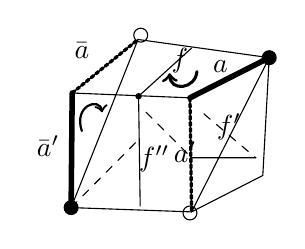
\begin{tikzpicture}[scale=.68,line cap=round]
\draw (0,0)--(2.25,-.08)--(3.58,.60)--(3.70,2.80)--(1.25,3.14)--(.02,2.14)--(2.22,2.05)--(2.25,-.08);
\draw[line width=2pt] (0,0)--(.02,2.14) (2.22,2.05)--(3.70,2.80);
\draw[densely dotted,line width=1.2pt] (.02,2.14)--(1.25,3.14) (2.22,2.05)--(2.25,-.08);
\draw (0,0)--(1.25,3.14) (2.25,-.08)--(3.70,2.80) (1.29,.03)--(1.26,2.08)--(2.25,2.98) (2.25,.93)--(3.45,.93);
\draw[dashed] (0,0)--(1.25,1.26) (1.40,1.78)--(2.25,.93) (2.48,1.75)--(3.45,.93);
\fill (0,0) circle (.14) (3.70,2.80) circle (.14) (1.26,2.08) circle (.06);
\draw (1.30,3.22) circle (.13) (2.22,-.10) circle (.13);
\draw[->,line width=1.1pt] (2.35,2.54) .. controls (2.32,2.21) and (1.85,2.16) .. (1.84,2.51);
\draw[->,thick] (.20,1.43) .. controls (.04,1.91) and (.53,2.07) .. (.58,1.78);
\node at (.20,2.93) {$\bar a$};\node at (-.43,1.14) {$\bar a'$};\node at (2.79,2.64) {$a$};
\node at (2.03,2.75) {$f$};\node at (1.55,.91) {$f''$};\node at (2.13,1.04) {$a'$};\node at (2.95,1.50) {$f'$};
\end{tikzpicture}}

\[
 \Sigma_a+\Sigma_{\bar a'}=\Sigma_{a'}+\Sigma_{\bar a}
\]

\[
 \begin{aligned}
 & &\tau_f+\tau_{f'}&=\Sigma_a & \tau_{\tilde f}+\tau_{\tilde f'}&=\Sigma_{\tilde a}=\Sigma_a\\
 &\unsure{4|7}\cdot3\cdot2=24=48/2\qquad &\tau_f\tau_{f'}&=\Pi_a & \tau_{\tilde f}\tau_{\tilde f'}&=\deleted{\unsure{\Pi}}\Pi_{\tilde a}=\Pi_a
 \end{aligned}
\]

donc $\{\tau_f,\tau_{f'}\}=\{\tau_{\tilde f},\tau_{\tilde f'}\}$

\figure{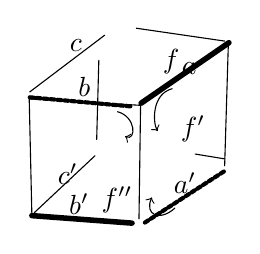
\begin{tikzpicture}[scale=.68,line cap=round]
\draw (0,.05)--(-.05,2.24)--(2.03,2.12)--(2,0) (2.02,2.12)--(3.67,3.30)--(3.60,.99) (3.6,3.32)--(1.95,3.56) (-.04,2.37)--(1.36,3.43);
\draw (.05,.12)--(1.18,1.18) (1.21,1.48)--(1.25,2.96) (3.05,1.21)--(3.60,1.12);
\draw[line width=2pt] (0,.06)--(1.87,-.08) (2.04,2.16)--(3.68,3.29);
\draw[densely dotted,line width=1.5pt] (-.04,2.27)--(1.85,2.10) (2.11,-.07)--(3.61,.90);
\draw[->] (1.60,2.0) .. controls (1.95,1.91) and (1.95,1.45) .. (1.74,1.54);
\draw[->] (2.62,2.43) .. controls (2.23,2.33) and (2.26,1.78) .. (2.35,1.64);
\draw[->] (2.67,.20) .. controls (2.38,-.06) and (2.1,.08) .. (2.24,.40);
\node at (.82,3.24) {$c$};\node at (.98,2.47) {$b$};\node at (2.60,2.94) {$f$};\node at (2.94,2.80) {$a$};
\node at (3.01,1.69) {$f'$};\node at (.67,.83) {$c'$};\node at (.88,.28) {$b'$};\node at (1.59,.35) {$f''$};\node at (2.86,.66) {$a'$};
\end{tikzpicture}}

\[
 \begin{aligned}
 \tau_f-\tau_{f''} &\unsure{=}\Sigma_a-\Sigma_{a'}=\Sigma_b-\Sigma_{b'} & \quad&\text{donc}\\
 \Sigma_a+\Sigma_{b'}&=\Sigma_b\unsure{-|+}\Sigma_{a'} &&
 \left\{\begin{aligned}\tau_f&=\tau_{\tilde f}\quad\text{\textcircled{ou}}\\
 \tau_f&=\tau_{\tilde f'}\end{aligned}\right.
 \end{aligned}
\]

\[
 \begin{aligned}
 \Sigma_a-\Sigma_{a'}&=\Sigma_c-\Sigma_{c'}\\
 \Sigma_a+\Sigma_{c'}&=\unsure{\Sigma_a|\Sigma_c}\unsure{-|+}\Sigma_c
 \end{aligned}
\]

$\Sigma_a$ ne dépend que de la direction de $a$ donc il \uline{n'y a que trois} \uline{valeurs} de $\Sigma_a$

de \unsure{=|même} il n'y a que trois valeurs de $\Pi_a$

\figure{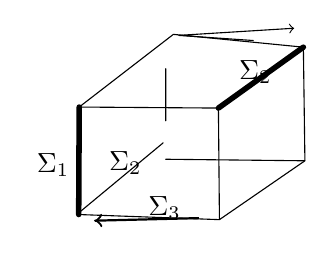
\begin{tikzpicture}[scale=.65,line cap=round]
\draw (0,0)--(2.75,-.10)--(4.42,1.05)--(4.39,3.27)--(1.85,3.52)--(.01,2.10)--(2.73,2.08)--(2.75,-.10);
\draw (.01,.04)--(1.65,1.40) (1.7,1.08)--(4.42,1.05) (1.70,1.83)--(1.70,2.85);
\draw[line width=2pt] (0,.0)--(.01,2.10) (2.73,2.08)--(4.39,3.27);
\draw[->,thick] (.32,-.12)--(2.35,-.07)--(.32,-.12);
\draw[->] (3.41,3.40)--(1.95,3.50)--(4.21,3.64);
\node at (-.50,.96) {$\Sigma_1$};\node at (.91,1.00) {$\Sigma_2$};\node at (1.68,.12) {$\Sigma_3$};\node at (3.45,2.79) {$\Sigma_2$};
\end{tikzpicture}}

$12$ relations de la forme $\Sigma_a+\Sigma_{a'}=\Sigma_b+\Sigma_{b'}$, \deleted{pour $\Sigma_a$ fixé} via opérations du groupe symétrique $\unsure{\mathfrak S|\mathscr S}_4$, elles se déduisent \unsure{l'une de l'autre|les unes des autres}
\scanpage{202}
\mspage{L 18}
% archive sheet number: 201

présenter un tel travail, que ce soient \deleted{\unsure{l}}\handwritten{\unsure{d|l}}es \inserted{\handwritten{manuels et autres}} textes didactiques\handwritten{,} \deleted{ou manuels,} ou \deleted{l}\handwritten{d}es articles \deleted{\unsure{ou|et}}\handwritten{et} mémoires\deleted{\unsure{,}} \deleted{ou de} originaux, ou les \deleted{exposés} cours oraux \deleted{ou}\handwritten{et} exposés de séminaires etc. Il y a, depuis des millénaires semblerait-il, depuis les\deleted{\unsure{ori}} origines mêmes de\deleted{\unsure{s}} la mathématique et des autres sciences\handwritten{,} \deleted{que nous cultivons,} une sorte de ``conspiration du silence'' autour de ces \deleted{aspect} ``\uline{inavouables} \uline{labeurs}'' qui préludent à l'éclosion de toute idée nouvelle, grande ou petite, venant renouveler notre connaissance d'une portion d\deleted{e}\unsure{e|u} \inserted{\handwritten{ce}} monde où nous vivons.

Pour tout dire, il semblerait que la répression de la connaissance de cet aspect là\deleted{\unsure{,}} \deleted{de plus \unsure{e}} ou de ce stade-là, le plus crucial de tous\deleted{\unsure{,}} dans le travail de découverte (et dans le travail créateur en général), soit à tel point efficace, à tel point in\deleted{\unsure{é}}tériorisé par ceux-là même qu\deleted{\unsure{u}}i pourtant connaissent un tel travail de première main, qu'on \deleted{\unsure{a|g}}jurerait souvent que même ceux-là \deleted{l'ont oublié} en ont éradiqué toute trace de leur souvenir conscient. Un peu comme dans une société puritaine à outrance, une femme aurait éradiqué de son souvenir, \deleted{toute trace} en relation à \inserted{chacun de} ces enfants qu'elle se fait un devoir de moucher et de torcher, le moment de l'étreinte (subie peut-être à contre-coeur) qui le\deleted{\unsure{s}} fit concevoir, les longs mois de la grossesse\deleted{\unsure{,}} (vécue comme \inserted{une} \unsure{inconvenante|inconvenance}) et les longues heures de l'accouchement (vécues comme un \inserted{\handwritten{peu ragoûtant}} martyre\handwritten{,} suivi enfin d\deleted{\unsure{e}}une délivrance).

Cette comparaison peut paraître \unsure{outéée|outrée}, et elle l'est peut-être, si je l'applique à \unsure{ce|le} que je me rappelle à présent de l'esprit que j'ai connu dans le milieu \inserted{mathématique} dont je faisais moi-même partie, il y a encore vingt ans. Mais \deleted{dans} j'ai pu me rendre compte, au cours de ma réflexion\deleted{\unsure{,}} \deleted{que dans les} dans Récoltes et Semailles, et de façon saisissante ces tout derniers mois surtout (avec l'écriture des Quatre Opérations), qu'il y a eu depuis mon départ de la scène mathématique une \deleted{dégra} dégradation stupéfiante dans l'esprit qui aujourd'hui fait loi dans les milieux que j'avais connus, et (me semble-t-il, dans une large mesure au moins) dans le monde mathématique en général. Il est possible même que mon départ, tant par ma personnalité mathématique très particulière que par les conditions qui ont entouré ce départ, ait agi comme un catalyseur dans une évolution qui était déjà en train de se faire ($^{\ast}$); \deleted{\illegible{1}} \inserted{\handwritten{évolution}} dont bien sûr je n'ai rien su percevoir (pas plus qu'\deleted{\unsure{a}}aucun de mes collègues et amis, à la seule exception peut-être de Claude Chevalley). L'aspect de cette dégradation \inserted{(parmi de nombreux autres ($^{\ast\ast}$))} auquel je pense ici est la \deleted{dérision, mépris} \mbox{m\,é\,p\,r\,i\,s}\quad\mbox{t\,a\,c\,i\,t\,e} , \deleted{prenant parfois les forme} quand ce n'est la dérision \deleted{\unsure{à} peine voilée,} \inserted{\handwritten{sans équivoque}} , vis à vis de ce qui, dans le travail (mathéma\unsure{t|q}i-
\scanpage{203}
% archive sheet number: 202

\figure{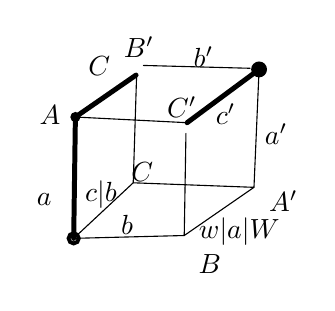
\begin{tikzpicture}[scale=.72,line cap=round]
\draw (0,0)--(1.95,.05)--(3.18,.90)--(3.27,2.98)--(2.0,2.04)--(.03,2.14)--(1.11,2.88) (1.23,3.05)--(3.11,3.00) (1.05,.98)--(1.11,2.88) (0,0)--(1.05,.98)--(3.18,.90) (1.95,.05)--(1.98,1.85);
\draw[line width=1.8pt] (0,0)--(.03,2.14)--(1.1,2.88) (2.0,2.04)--(3.27,2.98);
\fill (.03,2.14) circle (.09) (3.27,2.98) circle (.14);
\draw[line width=1.4pt] (0,0) circle (.09);
\node at (.45,3.04) {$\deleted{\unsure{C}}$};\node at (1.15,3.37) {$B'$};\node at (2.29,3.2) {$b'$};
\node at (-.42,2.18) {$A$};\node at (1.91,2.31) {$C'$};\node at (2.68,2.19) {$c'$};
\node at (3.57,1.84) {$a'$};\node at (-.52,.68) {$a$};\node at (.48,.78) {$\unsure{c|b}$};
\node at (1.21,1.17) {$C$};\node at (.94,.24) {$b$};\node at (2.40,-.45) {$B$};
\node at (2.92,.12) {$\unsure{w|a|W}$};\node at (3.70,.66) {$A'$};
\end{tikzpicture}}

% slanted
\margin{\tikz[baseline=(s.base)]\node[draw,ellipse,rotate=9,inner sep=4pt] (s) {Trop lourd};}

\[
 \begin{aligned}
 &\Sigma_{a\unsure{\prime}}\quad\Sigma_b\quad\Sigma_c\quad\Sigma_{AB'}\quad{}^{\unsure{-}}\Sigma_{BC'}\quad\Sigma_{CB'}\quad\Sigma_{CA'}\quad\Sigma_{AC'}\\
 &\Sigma_{a'}\quad\Sigma_{b'}\quad\Sigma_{c'}
 \end{aligned}
\]

\[
 \left\{\begin{aligned}
 \Sigma_a+\Sigma_{c'}&=\Sigma_{AB'}+\Sigma_{BC'}\\
 \Sigma_a+\Sigma_{b'}&=\Sigma_{AC'}+\Sigma_{CB'}\\
 \Sigma_b+\Sigma_{a'}&=\Sigma_{BC'}+\Sigma_{CA'}\\
 \Sigma_b+\Sigma_{c'}&=\Sigma_{BA'}+\Sigma_{AC'}\\
 \Sigma_c+\Sigma_{b'}&=\Sigma_{CA'}+\Sigma_{AB'}\\
 \Sigma_c+\Sigma_{a'}&=\Sigma_{CB'}+\Sigma_{BA'}\\[5pt]
 \left[\begin{aligned}
 \Sigma_a+\Sigma_{CA'}&=\Sigma_b+\Sigma_{CB'}\,.\\
 \Sigma_{a'}+\Sigma_{AC'}&=\Sigma_{b'}+\Sigma_{BC'}\\
 \Sigma_b+\Sigma_{AB'}&=\Sigma_c+\Sigma_{AC'}\,.\\
 \Sigma_{b'}+\Sigma_{BA'}&=\Sigma_{c'}+\Sigma_{CA'}
 \end{aligned}\right.&\\
 \Sigma_c+\Sigma_{BC'}&=\Sigma_a+\Sigma_{BA'}\,.\\
 \Sigma_{c'}+\Sigma_{CB'}&=\Sigma_{a'}+\Sigma_{AB'}
 \end{aligned}\right.
 \quad\vcenter{\hbox{\begin{tikzpicture}[overlay]
 \draw (-.5,3.5) .. controls (-.12,3.27) and (-.12,2.7) .. (-.55,2.28) .. controls (-.04,2.0) and (-.15,1.55) .. (-.48,1.08);
 \draw (-.49,3.06) .. controls (0,2.81) and (-.03,2.18) .. (-.54,1.78) .. controls (.05,1.53) and (.02,.76) .. (-.4,.44);
 \end{tikzpicture}}}
\]

$\exists\sigma$ avec $\sigma_{\underline a}+\sigma_{\underline b}+\sigma_{\underline c}=\sigma$ $\forall$ triple d'arêtes formant un ``demi hexagone''

\figure{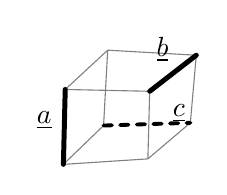
\begin{tikzpicture}[scale=.58,line cap=round]
\draw[thin,gray] (0,0)--(1.85,.12)--(2.78,.91)--(2.91,2.39)--(.97,2.50)--(.04,1.64)--(1.89,1.60)--(1.85,.12) (0,0)--(.88,.85)--(.97,2.50) (1.89,1.60)--(2.91,2.39);
\draw[line width=1.8pt] (0,0)--(.04,1.64) (1.89,1.60)--(2.91,2.39);
\draw[dashed,line width=1.4pt] (.88,.85)--(2.78,.91);
\node at (-.42,.96) {$\underline a$};\node at (2.17,2.52) {$\underline b$};\node at (2.53,1.12) {$\underline c$};
\end{tikzpicture}}

\[
 \Sigma_{a'}+\Sigma_{AC'}=\Sigma_{b'}+\deleted{\unsure{\Sigma}}\Sigma_{BC'}
\]

chacune des six dernières relations est conséquence des cinq autres, comme on voit en sommant, qui donne $0=0$!

\[
 \begin{aligned}
 &3(\Sigma_a+\Sigma_b+\Sigma_c+\Sigma_{a'}+\Sigma_{b'}+\Sigma_{c'})
 +(\Sigma_{CA'}+\Sigma_{AC'}\mathord{\text{---}}\,\mathord{\text{---}})\\
 &=(\Sigma_a+\Sigma_b\unsure{-|+}\Sigma_c+\Sigma_{a'}\unsure{-|+}\Sigma_{b'}\unsure{-|+}\Sigma_{c'})
 +3(\Sigma_{CA'}+\Sigma_{AC'}\quad)
 \end{aligned}
\]
\scanpage{204}
\mspage{L 17}
% archive sheet number: 203

\margin{\handwritten{\tikz{\draw (0,0)--(.28,0)--(.28,.32)--(.79,.33) (.32,0)--(.32,.32);}}}entrevu seulement et encore moins vu et touché, \deleted{pour} peu à peu se \deleted{dégager de son manteau de brumes, et se} \deleted{\inserted{d'ombre et}} décante\deleted{r} de l'impondérable, se dégage\deleted{r} de son manteau d'ombre et de brumes \deleted{et} \inserted{\handwritten{pour}} prendre forme et chair\deleted{\unsure{.}} \inserted{\handwritten{et poids}} \handwritten{...}

\deleted{Ce sont} \inserted{C'est} \deleted{ces stades} \inserted{cette partie}-là du travail, de piètre apparence pour ne pas dire \inserted{\handwritten{(bien des fois)}} foireux, qui \deleted{en représente\unsure{nt} aussi les plu} \inserted{en \deleted{sont} est aussi la \deleted{plus}\handwritten{partie}} \deleted{névralgique} \inserted{\handwritten{la plus délicate et la plus essentielle}} - celle où, véritablement, quelque chose de \mbox{n\,o\,u\,v\,e\,a\,u} fait son apparition, par l'effet d'une attention intense, d'une sollicitude, d'un respect pour cette chose fragile, infiniment délicate, sur le point de naître. C'est la partie créatrice entre toutes - celle\deleted{\unsure{s}} de la conception et d\deleted{e la}\handwritten{'une} \inserted{\handwritten{lente}} gestation \deleted{d'un fragile embryon} dans \deleted{\unsure{h}}\handwritten{l}es chaudes ténèbres de la matrice nourricière, \deleted{élaborant en silence} depuis l'invisible double gamète \deleted{initiale} originelle\handwritten{,} devenant \inserted{\handwritten{informe}} embryon et se transformant au fil des jours et des mois, par un travail obscur et intense, invisible et sans apparence, en un nouvel être en chair et en os.

\unsure{C'est|Cest} là aussi la partie \inserted{éminemment} ``yin'', ``féminine\deleted{\unsure{,}}'' du travail de découverte\handwritten{.}\deleted{-} \deleted{alors que la partie} \deleted{l}\handwritten{L}'aspect complémentaire ``yang'', ou masculin, s'apparenterait plutôt \deleted{\unsure{aux}} au travail à coups de marteaux ou de masse, sur un burin bien affûté ou sur un coin de bon acier \unsure{trëmpé|trempé}. L'un et l'autre aspect a sa raison d'être et sa fonction, en symbiose inséparable \inserted{l'un} avec l'autre - ou pour mieux dire, ce sont là \uline{l'épouse} et \uline{l'époux} du couple des deux forces cosmiques originelles, dont l'étreinte \deleted{\inserted{sans cesse} renouvelée fait} sans cesse renouvelée fait resurgir sans cesse les obscurs labeurs créateurs de la conception, de la gestation et de la naissance - de la naissance de \mbox{l'\,e\,n\,f\,a\,n\,t} , de la chose nouvelle.

La deuxième chose sur laquelle je sentais le besoin de m'exprimer, dans ma fameuse ``introduction'' \deleted{philosophique et} personelle et ``philosophique'' à un texte mathématique, c'était au sujet de la nature du travail créateur justement. Je me rendais compte, depuis des années, que cette nature était généralement \unsure{ignorée|ngnorée}, occultée par des clichés à tout venant et par des \inserted{\handwritten{répressions et des}} peurs ancestrales. A quel point il en est bien ainsi, je l'ai découvert \inserted{\handwritten{après seulement,}} \unsure{progressivement|progressigement}, \unsure{au|an} fil des jours et des mois, tout au cours de la réflexion et de ``l'enquêté'' poursuivie dans Récoltes et Semailles. C'est dès les tout débuts de cette réflexion, au mois de juin 198\deleted{\unsure{3}}\handwritten{3}, que je suis saisi pour la \unsure{première|premmère} fois (pour l'oublier \inserted{un peu} par la suite\handwritten{,}\deleted{ ...) par} \inserted{\handwritten{sous l'afflux des découvertes imprévues...) par}} la portée de ce fait d'anodine apparence, et pourtant asses stupéfiant, pour peu seulement qu'on s'y arrête tant soit peu: que cette partie ``créatrice entre toutes'' dont je viens de parler dans le travail de découverte, \uline{ne transparaît pratiquement nulle part} dans les textes \inserted{\handwritten{ou discours}} qui sont censés
\scanpage{205}
% archive sheet number: 204

\[
 \begin{aligned}
 &\text{\textcircled{4}}+\text{\textcircled{4}}\\[-2pt]
 &\quad+\text{\textcircled{6}}
 \end{aligned}
 \ \boxed{\begin{matrix}\text{\textcircled{$b_s$}}&\text{\textcircled{$c_s$}}\\
 \multicolumn{2}{c}{\text{\textcircled{$t_a$}}}\end{matrix}}
 \quad\begin{aligned}&(s\in S)\\ &(a\in A)\end{aligned}
 \qquad \text{avec}\quad b_s=b_{\bar s},\ c_s=c_{\bar s},\ b_a=t_{\bar a}
\]

\figure{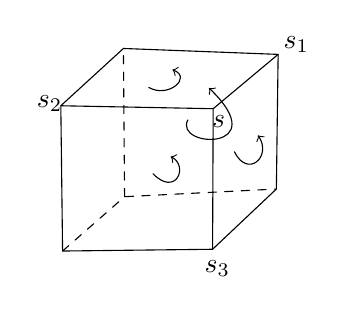
\begin{tikzpicture}[scale=.75,line cap=round]
\draw (0,0)--(2.54,.03)--(3.62,1.05)--(3.65,3.33)--(1.03,3.43)--(-.03,2.46)--(0,0);
\draw (-.03,2.46)--(2.55,2.41)--(3.65,3.33) (2.55,2.41)--(2.54,.03);
\draw[dashed] (0,0)--(1.05,.92)--(3.62,1.05) (1.05,.92)--(1.03,3.43);
\draw[->] (1.46,2.77) .. controls (1.79,2.58) and (2.20,2.94) .. (1.86,3.07);
\draw[->] (1.53,1.31) .. controls (1.92,.91) and (2.14,1.44) .. (1.83,1.60);
\draw[->] (2.91,1.68) .. controls (3.13,1.23) and (3.55,1.59) .. (3.31,1.96);
\draw[->] (2.12,2.22) .. controls (1.88,1.74) and (3.6,1.68) .. (2.48,2.76);
\node at (3.96,3.49) {$s_1$};\node at (-.22,2.5) {$s_2$};\node at (2.62,-.29) {$s_3$};\node at (2.64,2.20) {$s$};
\end{tikzpicture}}

Si $\delta(s)\inserted{\in I}$ est la diagonale qui passe par $s$, on a

\[
 \begin{aligned}b_s&=\operatorname{Tr}X_s\\c_s&=\det X_s\end{aligned}
\]

Si $\delta(a)\in\unsure{\mathcal P|P|\mathfrak P}_2(I)$ est \unsure{l'ens. des|l'une des} deux diagonales qui passent par les extr. de $a$, on a

\[
 \text{''}\qquad t_a=\operatorname{Tr}X_iX_j\inserted{=\operatorname{Tr}X_jX_i}
 \quad\text{si }\delta(a)=\{i,j\}
\]

\[
 4+4+\text{\textcircled{8}}\quad
 \underset{(s\in S)}{\boxed{\sigma_s,\pi_s,\text{\textcircled{$\unsure{T|\mathscr T|\tau|\mathbb T}_s$}}}}
\]

$s$ correspond \unsure{à|:} un triple $(i,j,\unsure{k|h})$ \unsure{à|:} perm. circulaire près

\[
 \begin{aligned}
 T_s&=\operatorname{Tr}X_iX_jX_k=\operatorname{Tr}X_{\deleted{\unsure{j}}j}X_kX_i=\operatorname{Tr}X_kX_iX_j\\
 T_{\bar s}&=\operatorname{Tr}X_kX_jX_i=\operatorname{Tr}X_jX_iX_k=\operatorname{Tr}X_iX_kX_j
 \end{aligned}
\]

\tikz[baseline=(a.base)]\node[draw,ellipse,inner sep=2pt] (a) {$4+4$ relations}; $\left(\begin{smallmatrix} R_s\\\wr\\R_{\bar s}\end{smallmatrix}\right)$

\[
 \boxed{\begin{aligned}
 \sigma_s&=\sigma_{\bar s}=T_s+T_{\bar s}\\
 \pi_s&=\pi_{\bar s}=T_s\cdot T_{\bar s}
 \end{aligned}}
\]

\[
 \begin{aligned}
 \sigma_s=\sigma_{\bar s}&=b_it_{jk}+b_jt_{ki}+b_kt_{ij}-b_ib_jb_k\\
 \deleted{\unsure{R_s=}}&=b_{s_1}t_{ss_1}+b_{s_2}t_{ss_2}+b_{s_3}t_{ss_3}-b_{s_1}b_{s_2}b_{s_3}
 \end{aligned}
\]

où $s_1,s_2,s_3$ sont les sommets adjacents à $s$

\[
 \begin{aligned}
 \unsure{\Pi|\pi}_s=\Pi_{\bar s}={}&t_{ss_1}t_{ss_2}t_{ss_3}
 +\deleted{(c_{s_1}t_{ss_1}+c_{s_2}t_{ss_2}+c_{s_3}t_{ss_3})}\\
 &\inserted{\bigl[c_{s_1}t_{ss_1}(t_{ss_1}-b_{s_2}b_{s_3})+
 c_{s_2}t_{ss_2}(t_{ss_2}-b_{s_3}b_{s_1})+
 c_{s_3}t_{ss_3}(\unsure{t_{s_3s_3}|t_{ss_3}|t_{s_1s_2}}-b_{s_1}b_{s_2})\bigr]}\\
 &+(b_{ss_1}^{2}c_{ss_2}c_{ss_3}+b_{ss_2}^{2}c_{ss_3}c_{ss_1}+b_{ss_3}^{2}c_{ss_1}c_{ss_2})
 \end{aligned}
\]

\[
 \text{\textcircled{6}}\quad
 \begin{array}{|c@{\ }l}\cline{1-1}
 \text{\textcircled{$T_f$}}\vrule & (f\in F)\\ \cline{2-2}
 \multicolumn{2}{|c|}{\sigma_a,\pi_a}\\\hline\end{array}\quad (a\in A)
\]

Si $f$ correspond à la permutation circulaire $(i,j,k,\unsure{l|\ell|e})$ de $I$, on a

\[
 T_f=\operatorname{Tr}X_iX_jX_kX_l=\deleted{\unsure{t_f=|\mathbb T_f=}}\operatorname{Tr}X_jX_kX_lX_i
 =\operatorname{Tr}X_kX_lX_iX_j=\operatorname{Tr}X_lX_iX_jX_k
\]

Si $f,f'$ sont adjacentes le long d'une arête $a=(s,t)$

\figure{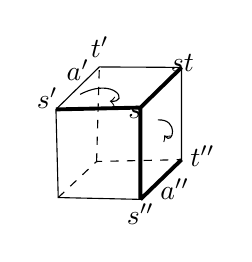
\begin{tikzpicture}[scale=.58]
\draw (0,0)--(1.8,-.04)--(2.7,.83)--(2.7,2.85)--(.90,2.86)--(-.05,1.93)--cycle;
\draw[line width=1.4pt] (-.05,1.93)--(1.8,1.97)--(2.7,2.85) (1.8,1.97)--(1.8,-.04) (1.8,-.04)--(2.7,.83);
\draw[dashed] (0,0)--(.84,.79)--(2.7,.83) (.84,.79)--(.90,2.86);
\draw[->] (.48,2.26) .. controls (1.23,2.65) and (1.57,2.08) .. (1.13,2.11);
\draw[->] (2.18,1.70) .. controls (2.65,1.73) and (2.52,1.13) .. (2.32,1.36);
\node at (-.24,2.18) {$s'$};\node at (.43,2.78) {$a'$};\node at (.91,3.29) {$t'$};\node at (2.72,2.95) {$\deleted{\unsure{s}}t$};
\node at (1.68,1.86) {$s$};\node at (1.8,-.37) {$s''$};\node at (2.55,.18) {$a''$};\node at (3.16,.91) {$t''$};
\end{tikzpicture}}

\diagram{\begin{tikzcd}[ampersand replacement=\&,column sep=1pt,row sep=3pt]
 f=(s\arrow[d]\&{,}t\arrow[d]\&{,}s'\arrow[d]\&{,}t')\arrow[d]\&{,}\quad f'=(t\arrow[d]\&{,}s\arrow[d]\&{,}t''\arrow[d]\&{,}s'')\arrow[d]\\
 i\&j\&k\&l\&j\&i\&k\&l
\end{tikzcd}}

\deleted{\unsure{Nb}} d'où $T_f=\operatorname{Tr}X_iX_j(X_kX_l)$, $T_{f'}=\operatorname{Tr}X_jX_i(X_kX_l)$, on a
\scanpage{207}
% archive sheet number: 206

\margin{\tikz[baseline=(r.base)]\node[draw,ellipse,inner sep=2pt] (r) {$\unsure{R_a|R_{ga}}$};\quad $12+12$ relations}

\[
 \boxed{\begin{aligned}
 \unsure{T|\mathscr T|\tau|\mathbb T}_f+T_{f'}&=\sigma_a\\
 T_fT_{f'}&=\Pi_a
 \end{aligned}}
\]

avec

\[
 \begin{aligned}
 \sigma_a={}&\operatorname{Tr}X_{\unsure{k|h}}X_{\unsure{l|\ell|e}}\,\operatorname{Tr}X_iX_j+
 \operatorname{Tr}X_i\,\operatorname{Tr}X_jX_kX_l+
 \operatorname{Tr}X_j\,\operatorname{Tr}X_kX_lX_i\\
 &-\operatorname{Tr}X_i\,\operatorname{Tr}X_j\,\operatorname{Tr}X_kX_l\\
 &\deleted{=\unsure{t_{st}t}\,'t}\\
 ={}&\underbrace{t_{a',a''}}_{\substack{\text{''}\\t_{a''}}}t_a+b_sT_s+b_tT_t-b_sb_tt_{a',a''}
 \end{aligned}
\]

$\Pi_a=\;\mathord{-}\,\mathord{-}\,\mathord{-}$ expression \inserted{un peu} plus compliquée en

\[
 \begin{aligned}
 &\deleted{\operatorname{Tr}X_i,\unsure{\mathrm d}}\quad b_i,c_i,b_j,c_j,t_{k\unsure{,|.}l},c_k,c_l\\
 &t_{i,j}\quad\underbrace{T_{jkl}}_{T_s}\quad\underbrace{T_{kli}}_{T_t}
 \end{aligned}
\]

$28$ variables $\overbrace{\overset{4}{b_s}\ \overset{4}{c_s}\ \overset{6}{t_a}}^{14}, \overbrace{\overset{8}{T_s},\ \overset{6}{T_f}}^{14}$

$32$ relations !
\scanpage{208}
% archive sheet number: 207

447 \quad ($^{\ast\handwritten{\ast}}$) Les deux autres livres sont les thèses de Jean Giraud et de \deleted{Monique} Monique Hakim (sur le formalisme des champs et de la \unsure{1|l}-cohomologie non commutative, et sur les schémas relatifs sur des topos annelés généraux).

448 \quad ($^{\ast}$) Cette citation (traduite) est extraite de la courte lettre (adressée au Dr. Peters) du 18 \unsure{février|févriier} l'an dernier, où je l'informais de ma décision de me retirer de l'``editorial board'' des Grundlehren. Le Dr. Peters avait en fait quitté déjà le Springer Verlag (il travaille à présent dans le Birkhäuser Verlag), et la correspondance s'est continuée avec le \deleted{\unsure{Dr.}} Dr. J. Heinze, en charge des Grundlehren dans la maison Springer\handwritten{.} \deleted{Verlag.} J'avais demandé\deleted{\unsure{e}} qu'une copie de ma lettre soit envoyée à chacun des co-éditeurs des Grundlehren (au nombre de dix-huit), et \unsure{avais|avaàs} réitéré cette prière au Dr Heinze\deleted{\unsure{,}} à deux reprises (en avril 84 et janvier 85) sans qu'il juge utile de me \deleted{dire} préciser si oui ou non elle avait été respectée (il \inserted{\handwritten{est}} appar\deleted{\unsure{aît|ait}}\handwritten{\unsure{ent|ut}} que \uline{non}). J'ai pris la peine d'envoyer moi-même une copie de \unsure{ma|la} lettre \deleted{de démission, avec quelques mots d'explication,} à chacun des dix-huit éditeurs, avec quelques mots d'explication \deleted{adressé} au sujet de cet envoi. \deleted{Parmi ces éditeurs, j'en conn} \inserted{Je} connais bien personnellement sept parmi \deleted{\unsure{ces}}\handwritten{eux}\handwritten{,} \deleted{éditeurs,} et \deleted{cinq entre eux} \handwritten{j'en} comptais \inserted{\handwritten{cinq}} parmi mes amis. Un seul \deleted{\unsure{(}} (Artin) a pris la peine de me répondre, et aucun apparemment \deleted{\unsure{n'a}}\handwritten{n'a} rien trouvé d'anormal \deleted{visà} (ne serait-ce que vis-à-vis de \mbox{l\,u\,i\,-\,m\,ê\deleted{\unsure{e}}m\,e} ) que la maison Springer n'ait pas \inserted{\handwritten{elle-même}} pris la peine de lui faire parvenir \deleted{elle-même} \deleted{au mois} (et dès le mois de février 1984) la lettre en question.

($^{\ast\ast\handwritten{\ast}}$) Ce sont les volumes n\textsuperscript{\uline{o}}s 288,340, 569, 589, 900.

($^{\ast\ast\ast\handwritten{\ast}}$) Comme je le précise dans l'avant-dernière note de b. de p. , le Dr. Peters a depuis quitté \inserted{\handwritten{le}} Springer Verlag pour Birkhäuser Verlag.

450 \quad ($^{\ast}$) \deleted{Voir mes observations \inserted{\unsure{(p.899)}} dans la sous-note ``Les double-sens - ou l'art de l'arnaque'' (n\textsuperscript{\uline{o}} 169$_7$), concernant} \inserted{\handwritten{Dans}} le fameux ``Fil d'Ariane'' (\deleted{à travers mon}\inserted{\handwritten{à travers SGA 4\unsure{, etc| et 5}}}) dans le volume nommé `` SGA $4\frac12$ '', \deleted{\unsure{on}} rien ne pourrait laisser supposer au lecteur que j'aie eu l'honneur de faire des exposés dans SGA 4 et SGA 5 (par contre, j'ai \inserted{\handwritten{bien}} eu celui de ``collaborer'' à ``SGA $4\frac12$ '' ...). \inserted{\handwritten{Voir à ce sujet mes observations dans la note ``Les double-sens - ou l'art de l'arnaque'' (n\textsuperscript{o} $169_{\unsure{7|2}}$), p. 899.}}

\unsure{451|452} \quad ($^{\ast}$) J'ai songé d'ailleurs aussi qu'il se pourrait bien que la situation se renverse, et que ce soit l'estimable entre\deleted{\unsure{m|p}}prise qui m'intente un procès, pour atteinte à sa réputation. \deleted{J'imagine que} \deleted{\unsure{c}}\handwritten{C}es gens ``au service de la \deleted{\unsure{s}}\handwritten{S}cience'', ils doivent être pointilleux sur ce chapitre \deleted{\unsure{en}} (du moment que c'est de \uline{leur} \deleted{propre} réputation qu'il s'agit ...).

452 \quad ($^{\ast}$) Cette idée-force de bâtir des ``maisons'', et qui soient bonnes ``pour tous'', a joué un rôle considérable dans mon oeuvre mathématique, et ceci depuis le début des années cinquante déjà. Cela a été l'expression concrète \deleted{de la ``pulsion de} \inserted{\handwritten{dans mon travail de}} ce que j'ai appelé la ``pulsion de service'' \deleted{en moi}, qui a fait partie (sans même que je la décèle avant la réflexion ``La clef du yin et du yang'') des \deleted{motivations profon} forces profondes donnant leur force vive à mon travail mathématique. L'archétype de la ``maison'' apparaît pour la première fois dans ma réflexion, \deleted{et avec} sans que je \inserted{ne} l'aie \deleted{entrev} pressent\inserted{\unsure{e}}\unsure{i}, et avec une grande force, dans la note \inserted{du 26 novembre} ``Yin le serviteur, et les nouveaux maîtres'' (n\textsuperscript{\uline{o}} 135).
